\documentclass{beamer}
\usetheme{CMU}

\usepackage{pgf,pgfarrows,pgfnodes,pgfautomata,pgfheaps,pgfshade}
\usepackage{amsmath,amssymb}
\usepackage[utf8]{inputenc}
\usepackage{colortbl}
\usepackage[english]{babel}
\usepackage{booktabs}
\usepackage{slpython}
\usepackage{underscore}

\author{Luís Pedro Coelho}
\institute{Programming for Scientists}

\graphicspath{{figures/}{figures/generated/}{images/}}

\newcommand*{\code}[1]{\textsl{#1}}


\title{Software Carpentry II: Programming Tools}
\begin{document}
\frame{\maketitle}

\begin{frame}[fragile]
\frametitle{Version Control}

If your laptop exploded, how many hours of work would you lose?
\end{frame}

\begin{frame}[fragile]
\frametitle{Advantages}
\begin{itemize}
\item Maintain project history.
\item Sync between computers.
\item Sync between project members.
\item \ldots
\end{itemize}
\end{frame}

\begin{frame}[fragile]
\frametitle{Subversion}
\begin{block}{Subversion: model}
\begin{enumerate}
\item Repository
\item Checkout
\item Commit
\end{enumerate}
\end{block}
\end{frame}

\begin{frame}[fragile]
\frametitle{Example}
\begin{enumerate}
\item Create a repository
\item Create a checkout
\item Edit
\item Commit
\end{enumerate}
\end{frame}

\begin{frame}[fragile]
\frametitle{Alternative: Simply Copying}

I can do this with file copying, no?

\pause

\begin{enumerate}
\item history
\item diffing
\item merging
\end{enumerate}
\end{frame}

\begin{frame}[fragile]
\frametitle{Do You Keep Old Versions Around?}
\begin{itemize}
\item bacteria.py
\item bacteria1.py
\item bacteria2.py
\item bacteria3.py
\item bacteria4.py
\item bacteria5.py
\item bacteriaold.py
\item bacteriaold2.py
\item bacteria.py2
\item \ldots
\end{itemize}
\end{frame}

\begin{frame}[fragile]
\frametitle{Do you explain your changes in the code?}

\begin{python}
def function(x,y,z):
    ...
    # Added 2/4/92 by LPC
    x = 0
    # Added 3/3/93 by XYZ
    x += 1
    # Added 8/23/97 by XYZ
    # Added 18/4/00 by MH
    print x
\end{python}
\end{frame}

\begin{frame}[fragile]
\frametitle{Diff'ing}

You have two versions of a file bacteria.py and bacteria2.py.

\bigskip
Find the changes.

\end{frame}
\begin{frame}[fragile]
\frametitle{Diffs \& Patches}

A diff is a patch.

\end{frame}

\begin{frame}[fragile]

\begin{block}{hello.py (1)}
\begin{python}
print 'Hello World'
\end{python}
\end{block}

\begin{block}{hello.py (2)}
\begin{python}
print 'Hello World'
print 'How are you?'
\end{python}
\end{block}

\begin{block}{diff (1)}
\begin{verbatim}
--- hello.py    2009-02-05 17:40:51.000000000 -0500
+++ hello2.py   2009-02-05 17:41:04.000000000 -0500
@@ -1 +1,2 @@
 print 'Hello World'
+print 'How are you doing?'
\end{verbatim}
\end{block}
\end{frame}

\begin{frame}[fragile]

\begin{block}{hello.py (1)}
\begin{python}
print 'Hello World'
\end{python}
\end{block}

\begin{block}{hello.py (2)}
\begin{python}
print 'Hello World'
print 'How are you?'
\end{python}
\end{block}

\begin{block}{diff (2)}
\begin{verbatim}
--- hello2.py   2009-02-05 17:41:04.000000000 -0500
+++ hello.py    2009-02-05 17:40:51.000000000 -0500
@@ -1,2 +1 @@
 print 'Hello World'
-print 'How are you doing?'
\end{verbatim}
\end{block}
\end{frame}

\begin{frame}[fragile]

\begin{block}{hello.py (1)}
\begin{python}
print 'Hello World'
\end{python}
\end{block}

\begin{block}{hello.py (2)}
\begin{python}
print 'Hello World'
print 'How are you?'
\end{python}
\end{block}

\begin{block}{diff (1)}
\begin{verbatim}
--- hello.py    2009-02-05 17:40:51.000000000 -0500
+++ hello2.py   2009-02-05 17:41:04.000000000 -0500
@@ -1 +1,2 @@
 print 'Hello World'
+print 'How are you doing?'
\end{verbatim}
\end{block}

\note{
    This repeats so that I can explain the concept, but I want to use this as the main example.
}
\end{frame}

\begin{frame}[fragile]
\frametitle{Example}

\begin{verbatim}
diff --git a/pyslic/preprocess/preprocesscollection.py b/pyslic/preprocess/preprocesscollection.py
index f060b8a..a8cd9ec 100644
--- a/pyslic/preprocess/preprocesscollection.py
+++ b/pyslic/preprocess/preprocesscollection.py
@@ -120,7 +120,10 @@ class FixIllumination(object):
         @see see
         '''
         assert self.S is not None
-        self.S /= self.S.min()
+        Smin = self.S.min()
+        if Smin == 0:
+            Smin = 1
+        self.S /= Smin
         # float96 is not always very well supported and we no longer need to sum up lots of numbers
         self.S = numpy.array(self.S,float)
\end{verbatim}

\end{frame}

\begin{frame}[fragile]
\frametitle{Merging}

\centering
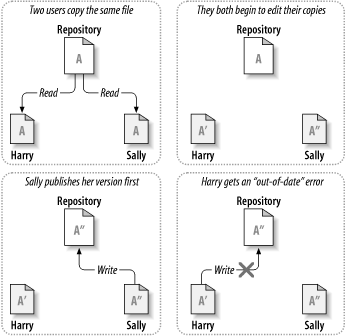
\includegraphics[width=.4\textwidth]{ch02dia4.png}

\begin{flushright}
(From the SVN Book --- link on course webpage, under \textit{Notes})
\end{flushright}

\end{frame}

\begin{frame}[fragile]
\frametitle{Merging (II)}

\centering
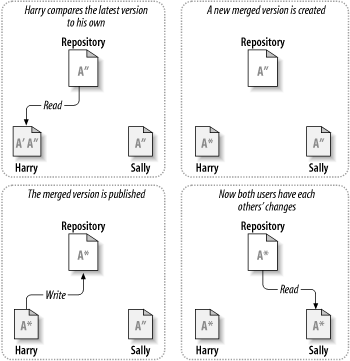
\includegraphics[width=.4\textwidth]{ch02dia5.png}

\begin{flushright}
(From the SVN Book --- link on course webpage, under \textit{Notes})
\end{flushright}

\end{frame}

\begin{frame}[fragile]
\frametitle{Version Control Etiquette}
\begin{itemize}
\item Don't commit over my commit.
\item Use the log.
\end{itemize}
\end{frame}

\begin{frame}[fragile]
\frametitle{Branches and Tags}
\begin{itemize}
\item Tag: name for revision.
\item Branch: multiple parallel tracks of development.
\end{itemize}

\end{frame}

\begin{frame}[fragile]
\frametitle{Defensive Programming}

Defensive programming means writing code that will catch bugs early.
\end{frame}

\begin{frame}[fragile]
\frametitle{Assertions}
\begin{python}
def stddev(values):
    '''
    S = stddev(values)

    Compute standard deviation
    '''
    assert len(S) > 0, 'stddev: got empty list.'
    ...
\end{python}
\end{frame}

\begin{frame}[fragile]
\frametitle{Assertions}

\begin{python}
def stddev(values):
    '''
    S = stddev(values)

    Compute standard deviation
    '''
    if len(S) <= 0:
        raise AssertionError(
            'stddev: got empty list.')
    ...
\end{python}

\end{frame}

\begin{frame}[fragile]
\frametitle{}

\begin{python}
def factorial(N):
    '''
    fN = factorial(N)

    Returns the factorial of N.

    N must be equal or greater than zero.
    '''
    if N == 0:
        return 1.
    return N * factorial(N-1)
\end{python}
\end{frame}

\begin{frame}[fragile]
\frametitle{Preconditions}

\begin{quote}
In computer programming, a precondition is a condition or predicate that must always be true just prior to the execution of some section of code.
\end{quote}

\begin{flushright}
(Wikipedia)
\end{flushright}

\end{frame}

\begin{frame}[fragile]
\frametitle{Preconditions}
\begin{block}{Other Languages}
\begin{itemize}
\item \alert{C/C++} \lstinline{#include <assert.h>}
\item \alert{Java} \lstinline{assert }\textit{pre-condition}
\item \alert{Matlab} \lstinline{assert()} (in newer versions)
\item \alert{\ldots} \ldots
\end{itemize}
\end{block}
\end{frame}

\begin{frame}[fragile]
\frametitle{Assertions Are Not Error Handling!}

\begin{itemize}
\item Error handling protect against outside events.
\item Assertions \alert{should never} be false.
\end{itemize}
\end{frame}


\begin{frame}[fragile]
\frametitle{Testing}

Do you test your code?

\end{frame}

\begin{frame}[fragile]
\frametitle{Unit Testing}

\begin{python}
def test_stddev_const():
    assert stddev([1]*100) < 1e-3

def test_stddev_positive():
    assert stddev(range(20)) > 0.
\end{python}

\end{frame}

\begin{frame}[fragile]
\frametitle{Nosetest}

Nose software testing framework:
\begin{itemize}
\item Tests are named \lstinline{test_}\textit{something}.
\item Conditions are \lstinline{assert}ed.
\end{itemize}

\end{frame}

\begin{frame}[fragile]
\frametitle{Software Testing Philosophies}

\begin{enumerate}
\item Test everything. Test it twice.
\item Write tests first.
\item Regression testing.
\end{enumerate}
\end{frame}

\begin{frame}[fragile]
\frametitle{Regression Testing}

Make sure bugs only appear once!

\end{frame}

\end{document}
